\section{Appendix B - Part 2}

\begin{lstlisting}[frame=single, label={lst:2a_PSD}, caption={MATLAB code to find the estimate of the Power Spectral Density of $S_{\psi_w}(w)$},captionpos=b]
%Part 2a
load('wave.mat')
x = psi_w(2,:)*pi/180;
window = 4096;
noverlap = [];
nfft = [];  
fs = 10;

% Power Spectral Density (PSD) function
[pxx,f] = pwelch(x, window, noverlap, nfft , fs); 

%Scaling to s/rad & rad/s
pxx = pxx/(2*pi);
f = f*2*pi;

\end{lstlisting}

\begin{figure}[H]
    \centering
    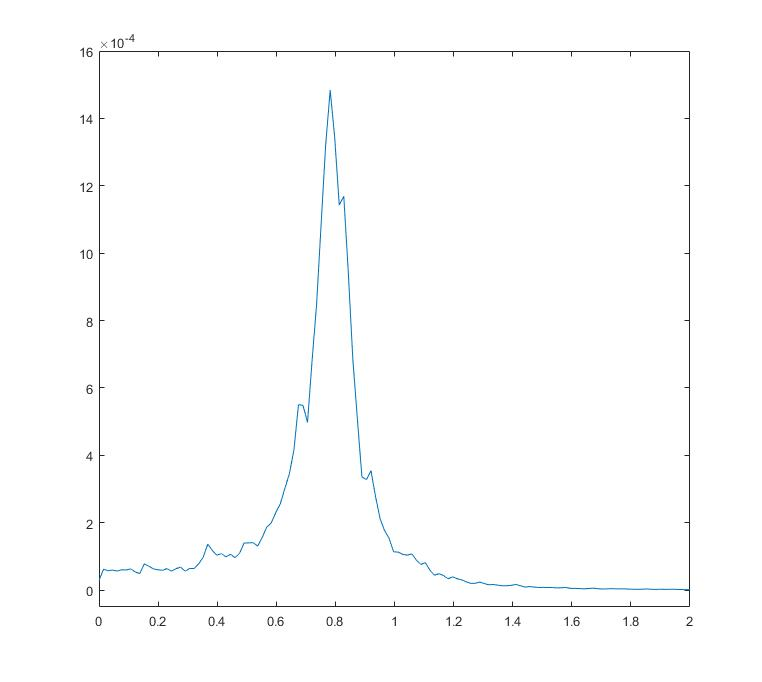
\includegraphics[width=0.8\textwidth]{Plots/2a_PSD.jpg}
    \caption{The plot shows the estimated Power Spectral Density (PSD) of the waves influencing our cargo ship. The x-axis is frequency (rad/s) and the y-axis is power (s/rad).}
    \label{fig: 2a_PSD}
\end{figure}

\begin{lstlisting}[frame=single, label={lst:2c_omegazero}, caption={MATLAB code to find $\omega_0$ from the estimated $S_{\psi_w}(w)$ combined with the MATLAB code in Listing (\ref{lst:2a_PSD}).},captionpos=b]
xmax = find(max(pxx) == pxx);
w_0 = f(xmax);
\end{lstlisting}

\begin{figure}[H]
    \centering
    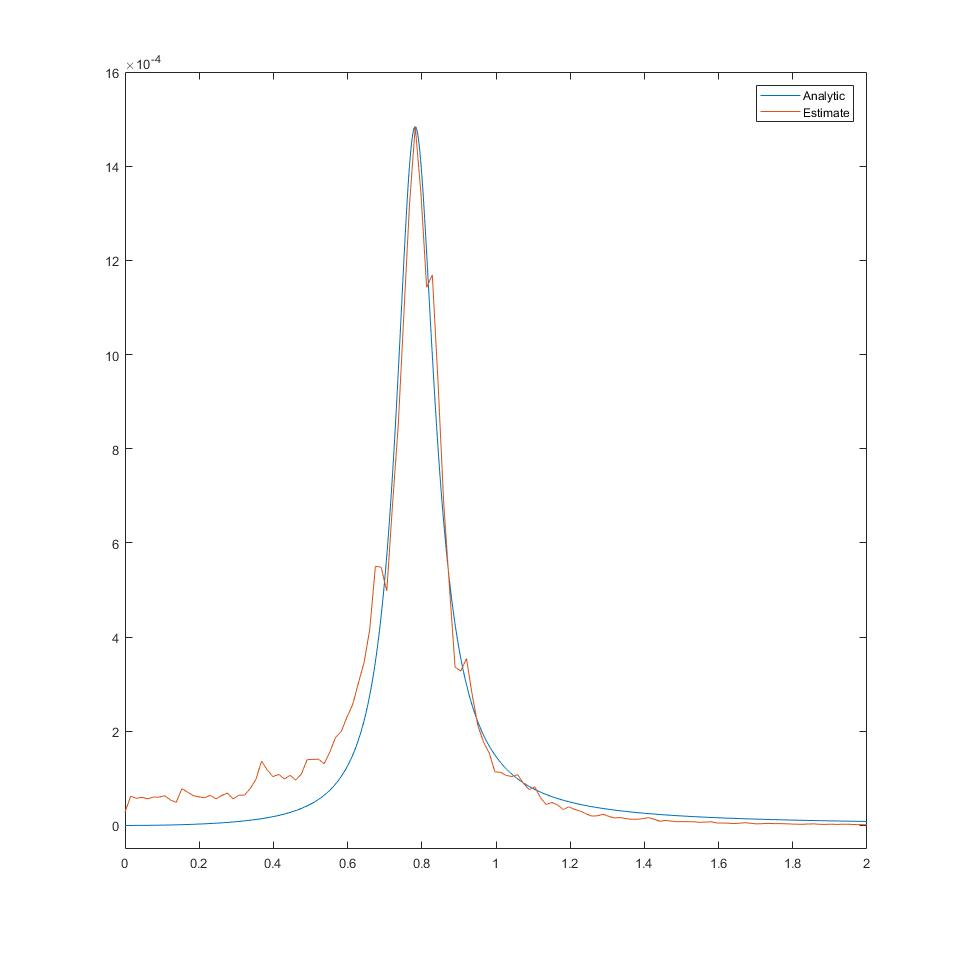
\includegraphics[width=1\textwidth]{Plots/2d_lambda_0082.jpg}
    \caption{The plot shows the analytical versus the estimated Power Spectral Density (PSD) of the waves influencing our cargo ship. The x-axis is frequency (rad/s) and the y-axis is power (s/rad).}
    \label{fig: 2d_lambda_0082}
\end{figure}